\documentclass[12pt]{article}
\usepackage{graphicx}
\usepackage[margin=1in]{geometry}
\usepackage{wrapfig}

\setlength{\parskip}{1em}

\begin{document}

\title{Security Venerabilities in Open Source Electronic Design Automation Software}
\author{Weston Braun}
\maketitle

\section{Introduction}
\label{S:1}
With the rise of the new "Maker" movement the number of open source software projects hosted online has rapidly rose. Work on these open source projects includes the wide exchange of files for electronic design automation (EDA) software, often from semi-anonymous users. The goal of this project is to take a look at some of these programs and see if this behavior represents a so far overlooked security risk. 

\section{Threat Model}
\label{S:2}
Open Source implies that the design files and code of a open source hardware project are publicly hosted. A typical hardware project consists of a schematic with its associated printed circuit board (PCB) layout, code for a microcontroller, and possibly 3D CAD files for an enclosure. Due to the crossover between the open source hardware and open source software communities, git is commonly used for version control with hosting through github or similar services. Project discovery happens though aggregator websites such as hackaday.com or dangerousprototypes.com, mailing lists, publications such as Make Magazine, or through search engines that index the project page. 

Once a user discovers a project they are often interested in viewing the schematic and PCB layout and to do so will download the project files. Unlike a software project where a makefile can be viewed in a text editor before running any commands from it, or code reviewed before being compiled, most EDA file formats are not designed for direct user readability. The easiest way to view the hardware design files is through the same EDA software that the project developer used, cross compatibility between different EDA programs is uncommon. 

The origins of these open source EDA programs date back to a time when public hosting of projects was less common and opening design files from the internet at large was not considered as part of the use case of the average user. However, with the current open source hardware community this is now expected behavior. It is believed that the difference between the original design philosophy of the software and the current usage presents an appreciable attack surface against an end users computer.  

As an additional threat, some PCB manufactures target towards the hobby and open source community have begun directly accepting EDA software files instead of the industry standard gerber files, which are a direct numerical representation of the PCB traces and holes. On the manufactures server a version of the EDA program will generate the gerber files directly to provide a preview for the end user and for the final manufacturing process. This presents an additional attack surface where an exploit in an EDA program can be used potential gain control of a server operated by a PCB manufacture. 


\section{Target Software}
\label{S:3}
Popular EDA software in the open source hardware community includes KiCad, Eagle, Altium, and gEDA. These programs all feature relatively the same work flow. They consist of a schematic capture tool where the user creates an electrical schematic using a library of component symbols. There is then an association between the schematic symbols and physical part footprints. Once the schematic is finished the user uses a second interface to create the PCB by positioning the physical component footprints and then drawing traces between them. 

Of the programs mentioned, both KiCad and gEDA are open source. KiCad is written in C++ and gEDA is written in C. In each of these programs the schematic capture tool and PCB layout tool are isolated as separate independent executables. KiCad is currently the more popular program with development funding being provided by CERN. However, both are available through the Debian repositories with gEDA using the package name 'pcb' and kicad using the package name 'kicad'. Which program to explore in depth was effected by the early results of the vulnerability search with gEDA becoming the focus of the project. 


\section{Vulnerability Search}
\label{S:4}
Because of the previously mentioned threat model of server side gerber file generation from design files, the search for vulnerabilities focused on the pcb layout component of KiCad and gEDA. The search for vulnerabilities consisted of manual code review added by static analysis and then fuzzing. The biggest attack surface was expected to be the parsers, which parses the human readable PCB layout / netlist consisting of part names, locations, and pin connections into the PCB data structure for display and modification. A vulnerability in the parser would allow for an exploit to execute with the user opening the file without any additional action. An additional attack surface discovered in this process was the user interface itself. Malicious strings can make it through the parser and exploit display formatting functions. 

\subsection{Static Analysis / Code Review}
KiCad and gEDA both have significant code bases, consisting of a parser for file input, functions to modify the schematic or PCB, and display formatting and GUI. According to the CLOC utility, the KiCad PCB utility, pcbnew, has a codebase of 109,386 lines of C++ code while the codebase for the gEDA pcb utility, pcb, has 102,379 lines of C code. This size of this codebase makes full manual review difficult. A static analysis tool, which searches through the code for potentially unsafe functions or pointer arithmetic was used to reduce this search. Flawfinder, a utility available in the Debian package manager, is capable of parsing C and C++ code and proved suitable for this purpose. 

Running on the KiCad pcbnew codebase Flawfinder yielded 104 potential security vulnerabilities. Upon manual review of these hits it was revealed that as a class of vulnerabilities, string based buffer overflows were in large prevented through the consistent use of the wxString library, which dynamically resizes strings, preventing direct buffer overflows. There were some potentially interesting issues relating to race conditions on file access. However, they are not applicable to the threat model of exploitation via a malicious file. Due to the more modern and better maintained codebase and use of C++ features that make buffer overflows more difficult it was decided at this point that gEDA would present a more promising target. 

When run on the gEDA pcb codebase Flawfinder yielded 487 potential security vulnerabilities. Upon review of these hits two buffer overflows relating to the pin display names were discovered. Both of these are triggered by user action. One is a heap overflow triggered by the user moving the mouse over a pin which automatically pops up a dialog box showing the pin name. A stack overflow is achievable through a dialog box used by the change pin name tool.

\subsection{Fuzzing}
\subsection{Implementation} 
Fuzzing was used with the hope of finding errors in the gEDA pcb parser which could be used in an exploit. The fuzzer of choice, AFL-fuzz, requires an instrumented binary compiled afl-gcc that will terminate on its own, and one or more minimal input files to fuzz. An example PCB layout was reduced down to the minimal feature set and the gEDA pcb source was modified to terminate after parsing the input file. Initial fuzzing attempts on a test VM were very slow (4 executions per second) due to CPU limitations and the GUI launching with every execution. Attempts to were made to separate the parsing functions from the GUI to speed up execution but the parsing functions required the memory structures initialized by the GUI library. Bypassing this would have required a rewrite of part of the GUI library which was deemed beyond the scope of the project. Using a dedicated machine with a fake x11 display driver improved performance and allowed for approximately 100 executions per second. The fuzzing was allowed to run for 24 hours to achieve acceptable path coverage. 

\subsubsection{Results}
Fuzzing yielded 340 pcb files which would crash the gEDA pcb program when opened. This ended up being significantly more files than were practical to review within the scope of the project. A random subset of the files were manually with reviewed and analyzed with gdb. This revealed a significant number of heap corruption errors, some segfaults, and a stack overflow. It was discovered with the heap corruption errors the program crash was occurring at the point of the out of bounds memory write but when the pcb buffer was passed to free. Valgrind was used to profile the program when parsing these files and discover the actually location of the heap corruption. 

The most interesting errors that were discovered via fuzzing were a stack overflow and a sefault write that could possibly be utilized as an arbitrary memory write. Analysis of more vulnerabilities discovered by the parser is hosted on the projects github page.  
\section{Exploit}
\label{S:5}
Even though none of the vulnerabilities that were discovered would have allowed for the creation of an exploit that would work against the version of gEDA pcb program available from the package manger, it was decided that a proof of concept exploit should be developed that could run against an unmodified codebase but with the standard protections disabled. It was decided to utilize the stack based buffer overflow of the pin display number that was discovered via static analysis. This stack overflow is triggered through the dialog box for changing the pin name, which is shown in figure \ref{fig:rename-gui}. 
\begin{wrapfigure}{R}{0.3\textwidth}
\centering
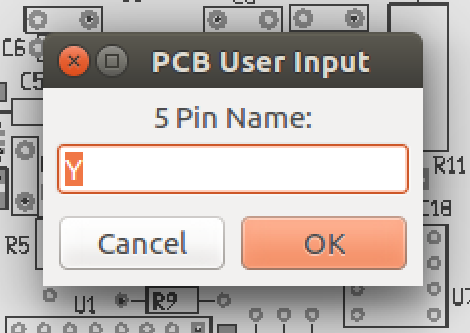
\includegraphics[width=0.3\textwidth]{images/rename-gui-cropped.png}
\caption{Pin Renaming Dialog Box}
\label{fig:rename-gui}
\end{wrapfigure}

The exploit runs with the address space randomization disable, stack canaries disabled, fortify source disabled, and stack execution enabled. It would have also been possible to produce a version which did not require an executable stack and instead by redirecting the program control flow to call libc functions. To bypass address space randomization an address leakage would be needed which was not found in the code analysis or fuzzing. 

To create the exploit a python script was created that inserts the shellcode and execution addresses as the pin number of a specific pin in an example pcb layout. Once the use opens this file and attempts to rename that pin the shellcode will be executed. Due to the presence of non display characters in the buffer the payload fails to display via the gui, hiding the attack from the user. Figure \ref{fig:exploit-gui} shows the pin renaming dialog when the exploit is underway. The example shellcode used for this exploit is borrowed from the 6.858 course material and launches a shell, but could in practice could be any malicious action. 

\begin{wrapfigure}{R}{0.3\textwidth}
\centering
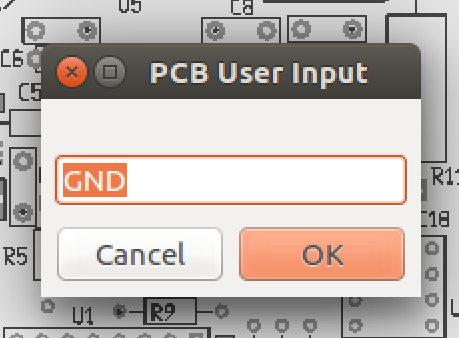
\includegraphics[width=0.3\textwidth]{images/exploit-gui-cropped.png}
\caption{Dialog Box During Exploit}
\label{fig:exploit-gui}
\end{wrapfigure}

\section{Future Work}
\label{S:6}
Future work for this project would include writing replacement functions for the GUI library to allow for faster fuzzing and work on utilities to better process the results of the fuzzing. The fuzzing yielded 340 unique crashes but due to time constraints it was only possible to go though a subset of them. Having to run GDB for each crash file and manually review the code to discovered the cause was extremely time consuming. It may be difficult to automate the process of judging the utility of a vulnerability but even some basic classification save time. It is highly likely that promising vulnerabilities were missed in the sheer volume of unique crashes. 

\section{Conclusion}
\label{S:7}
Although this project did not result in an exploit which works on an EDA program installed directly from the release website or package manager it did illustrate the validity of the threat model presented by the open sharing of open source hardware design files. Given that vulnerabilities were found that were mitigated only by toolchain and OS protections it is quite likely further analysis could find a fully exploitable vulnerability. Additionally, given that the gEDA project dates back to 1998 it is possible that the exploit that was created would have worked on some past computer. The author will sure to be careful in opening any CAD or EDA files sourced from the internet in the future. 



\end{document}